\section{Equivalence Relations} \label{S:equivrelations}
%\markboth{Chapter~\ref{C:equivrelations}. Equivalence Relations}{\ref{S:equivrelations}. Equivalence Relations}
\setcounter{previewactivity}{0}
%
%\begin{previewactivity}[\textbf{Directed Graphs and Relations}] \label{PA:directedgraphs} \hfill \\
If  $A$  is a (small) finite set, a relation  $R$  on  $A$  can be specified by simply listing all the ordered pairs in  $R$.  For example,  if  $A = \left\{ {1, 2, 3, 4} \right\}$, then 
\[
R = \left\{ {( {1, 1} ), ( {4, 4} ), ( {1, 3} ), ( {3, 2} ), ( {1, 2} ), ( {2, 1} )} \right\}
\]
is a relation  on  $A$.  A convenient way to represent such a relation is to draw a point in the plane for each of the elements of  $A$  and then for each  $\left( {x, y} \right) \in R$ (or  
$x \mathrel{R} y$),  we draw an arrow starting at point $x$  and pointing to point $y$.  If  
$\left( {x, x} \right) \in R$ (or  $x \mathrel{R} x$), we draw a loop at the point  $x$.  The resulting diagram is called a \textbf{directed graph} \label{directedgraph}
\index{directed graph}%
 or a \textbf{digraph}.
\index{digraph}%
  The diagram in Figure~\ref{fig:dirgraph} is a digraph for the relation  $R$.

\begin{figure}[h]
\begin{center}
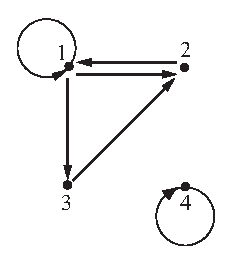
\includegraphics{figps-prev72digraph.eps}
\caption{Directed Graph for a Relation} \label{fig:dirgraph}
\end{center}
\end{figure}

In a directed graph, the points are called the \textbf{vertices}.  So each element of  $A$  corresponds to a \textbf{vertex}.
\index{vertex}%
\index{directed graph!vertex}%
  The arrows, including the loops, are called the \textbf{directed edges}
\index{directed edge}%
\index{directed graph!directed edge}%
 of the directed graph.

\begin{enumerate}
\item Let  $A = \left\{ {1, 2, 3, 4} \right\}$ and  
$R = \left\{ {( {1, 1} ), ( {2, 2} ), ( {3, 3} ), ( {4, 4} ), ( {1, 3} ), ( {3, 2} )} \right\}$.  Draw a digraph for this relation and then determine whether the following statements are true or false.  \label{PA:directedgraphs1}

\begin{enumerate}
  \item For each  $x \in A$,  $x \mathrel{R} x$.

  \item For every  $x, y \in A$, if  $x \mathrel{R} y$, then  $y \mathrel{R} x$.

  \item For every  $x, y, z \in A$, if  $x \mathrel{R} y$ and  $y \mathrel{R} z$, then  
                   $x \mathrel{R} z$.
\end{enumerate}

\item Let  $A = \left\{ {1, 2, 3, 4} \right\}$ and  
$S = \left\{ {( {1, 1} ), ( {1, 4} ), ( {2, 4} ), ( {4, 1} ), ( {4, 2} )} \right\}$.  Draw a digraph for this relation and then determine whether the following statements are true or false.

\begin{enumerate}
  \item For each  $x \in A$,  $x \mathrel{S} x$.

  \item For every  $x, y \in A$, if  $x \mathrel{S} y$, then  $y \mathrel{S} x$.

  \item For every  $x, y, z \in A$, if  $x \mathrel{S} y$ and  $y \mathrel{S} z$, then  
                   $x \mathrel{S} z$.
\end{enumerate}
\end{enumerate}
\end{previewactivity}
\hbreak
%
\begin{previewactivity}[\textbf{Properties of Relations}] \label{PA:propsofrelaitons} \hfill \\
In Preview Activity~\ref{PA:directedgraphs}, the same three questions were asked about two different relations on the set $A = \left\{ {1, 2, 3, 4} \right\}$.  These were questions about certain properties of relations, and these properties occur frequently enough to warrant names.

\begin{defbox}{ref-sym-trans}{Let  $A$  be a nonempty set and let  $R$  be a relation on  $A$.
\begin{itemize}
\item The relation  $R$  is \textbf{reflexive on}
\index{reflexive}%
\index{relation!reflexive on}%
 $\boldsymbol{A}$  provided that for each  
$x \in A$,  $x \mathrel{R} x$ or, equivalently,  $\left( {x, x} \right) \in R$.

\item The relation  $R$  is \textbf{symmetric}
\index{symmetric}%
\index{relation!symmetric}%
  provided that for every  $x, y \in A$,  if  
$x \mathrel{R} y$, then  $y \mathrel{R} x$ or, equivalently, for every  $x, y \in A$,  if  $\left( {x, y} \right) \in R$, then  $\left( {y, x} \right) \in R$.

\item The relation  $R$  is \textbf{transitive}
\index{transitive}%
\index{relation!transitive}%
  provided that for every $x, y, z \in A$,  if  $x \mathrel{R} y$ and  $y \mathrel{R} z$, then  $x \mathrel{R} z$ or, equivalently, for every  $x, y, z \in A$,  if  $\left( {x, y} \right) \in R$ and $\left( {y, z} \right) \in R$, then  $\left( {x, z} \right) \in R$.
\end{itemize}
}
\end{defbox}

\noindent
Define the relations  $\sim$  and  $ \approx $  on  $\Q$  as follows:  For all $a, b \in Q$,
\begin{itemize}
\item $a \sim b$  if and only if  $a - b \in \Z $.	

\item $a \approx b$  if and only if  $a + b \in \Z$.
\end{itemize}

\noindent
For example, $\dfrac{3}{4} \sim \dfrac{7}{4}$ since $\dfrac{3}{4} - \dfrac{7}{4} = -1$, and 
$\dfrac{3}{4} \not  \approx \dfrac{7}{4}$ since $\dfrac{3}{4} + \dfrac{7}{4} = \dfrac{5}{2}$.

\begin{enumerate}
\item Is the relation  $\sim$  a reflexive relation on  $\Q$?  Is it a symmetric relation?  Is it a transitive relation? 

\item Is the relation  $ \approx $  a reflexive relation on  $\Q$?  Is it a symmetric relation?  Is it a transitive relation?
\end{enumerate}
\end{previewactivity}
\hbreak
%
\pagebreak
\begin{previewactivity}[\textbf{Review of Congruence Modulo} $\boldsymbol{n}$]\label{PA:reviewofcongruence} \hfill
\begin{enumerate}
\item Let  $a, b \in \mathbb{Z}$ and let  $n \in \mathbb{N}$.  On page~\pageref{congruence} of Section~\ref{S:directproof}, we defined what it means to say that  $a$  is congruent to  $b$  modulo  $n$.  Write this definition and state two different conditions that are equivalent to the definition.

\item %Let  $a, b \in \mathbb{Z}$ and let  $n \in \mathbb{N}$.  We use  
%$a \equiv b \pmod n$ as a notation for  ``$a$  is congruent to  $b$  modulo  $n$.''  
Explain why congruence modulo  $n$  is a relation on  $\mathbb{Z}$.

\item Carefully review Theorem~\ref{T:modprops} and the proofs given on page~\pageref{T:modprops} of Section~\ref{S:directproof}.  In terms of the properties of relations introduced in Preview Activity~\ref{PA:propsofrelaitons}, what does this theorem say about the relation of congruence modulo  $n$  on the integers?

\item Write a complete statement of Theorem~\ref{T:congtorem} on page~\pageref{T:congtorem} and Corollary~\ref{C:congtorem}.

\item Write a proof of the symmetric property for congruence modulo  $n$.  That is, prove the following:

\begin{list}{}
\item Let  $a, b \in \mathbb{Z}$ and let  $n \in \mathbb{N}$.  If  
$a \equiv b \pmod n$, then  $b \equiv a \pmod n$.
\end{list}

\end{enumerate}
\end{previewactivity}
\hbreak




\endinput


\begin{center}
\setlength{\unitlength}{0.5cm}
\begin{picture}(8,8)
\put(2,2){\circle*{.25}}
\put(2,6){\circle*{.25}}
\put(6,2){\circle*{.25}}
\put(6,6){\circle*{.25}}

\put(1.8,1.2){3}
\put(5.8,1.2){4}
\put(5.8,6.4){2}
\put(1.6,6.3){1}

\put(2.3,5.8){\vector(1,0){3.4}}
\put(5.7,6.2){\vector(-1,0){3.4}}
\put(2.2,2.2){\vector(1,1){3.4}}
\put(2,5.7){\vector(0, -1){3.4}}

\put(6,1){\circle{2}}
\put(6,2){\vector(1,0){0}}

\put(1.3,6.7){\circle{2}}
\put(2,6){\vector(1,1){0}}

\end{picture}
\end{center}

In Preview Activity~(\ref{PA:directedgraphs}), the same three questions were asked about two different relations on the set $A = \left\{ {1, 2, 3, 4} \right\}$.  These were questions about certain properties of relations, and these properties occur frequently enough to warrant names.

\begin{defbox}{ref-sym-trans}{Let  $A$  be a nonempty set and let  $R$  be a relation on  $A$.
\begin{itemize}
\item The relation  $R$  is \textbf{reflexive on}
\index{reflexive}%
\index{relation!reflexive on}%
 $\boldsymbol{A}$  provided that for each  
$x \in A$,  $x \mathrel{R} x$ or, equivalently,  $\left( {x, x} \right) \in R$.

\item The relation  $R$  is \textbf{symmetric}
\index{symmetric}%
\index{relation!symmetric}%
  provided that for every  $x, y \in A$,  if  
$x \mathrel{R} y$, then  $y \mathrel{R} x$ or, equivalently, for every  $x, y \in A$,  if  $\left( {x, y} \right) \in R$, then  $\left( {y, x} \right) \in R$.

\item The relation  $R$  is \textbf{transitive}
\index{transitive}%
\index{relation!transitive}%
  provided that for every $x, y, z \in A$,  if  $x \mathrel{R} y$ and  $y \mathrel{R} z$, then  $x \mathrel{R} z$ or, equivalently, for every  $x, y, z \in A$,  if  $\left( {x, y} \right) \in R$ and $\left( {y, z} \right) \in R$, then  $\left( {x, z} \right) \in R$.
\end{itemize}
}
\end{defbox}

Let  $U$  be a finite, nonempty set and let  $\mathcal{P}\left( U \right)$ be the power set of  $U$.  Define the relations  $\sim$  and  $ \approx $  on  $\mathcal{P}\left( U \right)$  as follows:

\vskip10pt
\noindent
For  $A, B \in P\left( U \right)$,
\begin{itemize}
\item $A \sim B$  if and only if  $A \cap B = \emptyset $.	That is,  the ordered pair  
$\left( {A, B} \right)$  is in the relation  $\sim$  if and only if  $A$  and  $B$  are disjoint.

\item $A \approx B$  if and only if  $\left| A \right| = \left| B \right|$.	That is, the ordered pair  $\left( {A, B} \right)$  is in the relation  $ \approx $  if and only if  $A$  and  $B$  have the same cardinality (same number of elements).
\end{itemize}

\begin{enumerate}
\item Is the relation  $\sim$  a reflexive relation on  $\mathcal{P}\left( U \right)$?  Is it a symmetric relation?  Is it a transitive relation? 

\item Is the relation  $ \approx $  a reflexive relation on  $\mathcal{P}\left( U \right)$?  Is it a symmetric relation?  Is it a transitive relation?
\end{enumerate}
\end{previewactivity}
\hbreak


\begin{previewactivity}[\textbf{Properties of Relations}] \label{PA:propsofrelaitons} \hfill \\
In previous mathematics courses, we have worked with the equality relation.  For example, let $R$ be the relation on $\Z$ defined as follows:  For all $a, b \in \Z$,  $a \mathrel{R} b$ if and only if $a = b$.  We know this equality relation on $\Z$ has the following properties:
\begin{itemize}
  \item For each $a \in \Z$, $a = a$ and so $a \mathrel{R} a$.
  \item For all $a, b \in \Z$, if $a = b$, then $b = a$.  That is, if $a \mathrel{R} b$, then $b \mathrel{R} a$.
  \item For all $a, b, c \in \Z$, if $a = b$ and $b = c$, then $a = c$.  That is, if $a \mathrel{R} b$ and 
         $b \mathrel{R} c$, then $a \mathrel{R} c$.
\end{itemize}
In mathematics, when something satisfies certain properties, we often ask if other things satisfy the same properties.  Before investigating this, we will give names to these properties.

%In Beginning Activity~\ref{PA:directedgraphs}, the same three questions were asked about two different relations on the set $A = \left\{ {1, 2, 3, 4} \right\}$.  These were questions about certain properties of relations, and these properties occur frequently enough to warrant names.

\begin{defbox}{ref-sym-trans}{Let  $A$  be a nonempty set and let  $R$  be a relation on  $A$.
\begin{itemize}
\item The relation  $R$  is \textbf{reflexive on}
\index{reflexive}%
\index{relation!reflexive on}%
 $\boldsymbol{A}$  provided that for each  
$x \in A$,  $x \mathrel{R} x$ or, equivalently,  $\left( {x, x} \right) \in R$.

\item The relation  $R$  is \textbf{symmetric}
\index{symmetric}%
\index{relation!symmetric}%
  provided that for every  $x, y \in A$,  if  
$x \mathrel{R} y$, then  $y \mathrel{R} x$ or, equivalently, for every  $x, y \in A$,  if  $\left( {x, y} \right) \in R$, then  $\left( {y, x} \right) \in R$.

\item The relation  $R$  is \textbf{transitive}
\index{transitive}%
\index{relation!transitive}%
  provided that for every $x, y, z \in A$,  if  $x \mathrel{R} y$ and  $y \mathrel{R} z$, then  $x \mathrel{R} z$ or, equivalently, for every  $x, y, z \in A$,  if  $\left( {x, y} \right) \in R$ and $\left( {y, z} \right) \in R$, then  $\left( {x, z} \right) \in R$.
\end{itemize}
}
\end{defbox}
Before exploring examples, for each of these properties, it is a good idea to understand what it means to say that a relation does not satisfy the property.  So let  $A$  be a nonempty set and let  $R$  be a relation on  $A$. 
\begin{enumerate}
\item Carefully explain what it means to say that the relation  $R$  is not reflexive on the set  $A$.

\item Carefully explain what it means to say that the relation  $R$  is not symmetric.

\item Carefully explain what it means to say that the relation  $R$  is not transitive.
\end{enumerate}
To illustrate these properties, we let  $A = \left\{ {1, 2, 3, 4} \right\}$ and define the relations $R$ and $T$ on $A$ as follows:
\begin{align*}
R &= \left\{ {( {1, 1} ), ( {2, 2} ), ( {3, 3} ), ( {4, 4} ), ( {1, 3} ), ( {3, 2} )} \right\} \\
T &= \left\{ {( {1, 1} ), ( {1, 4} ), ( {2, 4} ), ( {4, 1} ), ( {4, 2} )} \right\}
\end{align*}
\setcounter{oldenumi}{\theenumi}
\begin{enumerate} \setcounter{enumi}{\theoldenumi}
\item Draw a directed graph for the relation $R$. Then explain why the relation $R$ is reflexive on $A$, is not symmetric, and is not transitive.
\item Draw a directed graph for the relation $T$.  Is the relation $T$ reflexive on $A$?  Is the relation $T$ symmetric?  Is the relation $T$ transitive?  Explain. 
\end{enumerate}
%   We then see that the relation $R$ is reflexive on $A$.  (Why?)  However:
%\begin{itemize}
%  \item The relation $R$ is not symmetric since $(1, 3) \in R$ but $(3, 1) \notin R$.  ($1 \mathrel{R} 3$ but $3 \not \negthickspace \negthinspace \mathrel{R} 1$.)
%  \item The relation $R$ is not transitive since $(1, 3) \in R$ and $(3, 2) \in R$, but $(1, 3) \notin R$.  ($1 \mathrel{R} 3$ and $3 \mathrel{R} 2$ but $3 \not \negthickspace \negthinspace \mathrel{R} 2.)$
%\end{itemize}
%\begin{enumerate}
%  \item Let  $A = \left\{ {1, 2, 3, 4} \right\}$ and  
%$S = \left\{ {( {1, 1} ), ( {1, 4} ), ( {2, 4} ), ( {4, 1} ), ( {4, 2} )} \right\}$.  Draw a digraph for this relation and then determine if the relation $S$ is reflexive on $A$, if the relation $S$ is symmetric, and if the relation $S$ is transitive.
%\end{enumerate}
%
%\noindent
%Define the relations  $\sim$  and  $ \approx $  on  $\Q$  as follows:  For all $a, b \in Q$,
%\begin{itemize}
%\item $a \sim b$  if and only if  $a - b \in \Z $.	
%
%\item $a \approx b$  if and only if  $a + b \in \Z$.
%\end{itemize}
%
%\noindent
%For example, $\dfrac{3}{4} \sim \dfrac{7}{4}$ since $\dfrac{3}{4} - \dfrac{7}{4} = -1$, and 
%$\dfrac{3}{4} \not  \approx \dfrac{7}{4}$ since $\dfrac{3}{4} + \dfrac{7}{4} = \dfrac{5}{2}$.
%
%\begin{enumerate}
%\item Is the relation  $\sim$  a reflexive relation on  $\Q$?  Is it a symmetric relation?  Is it a transitive relation? 
%
%\item Is the relation  $ \approx $  a reflexive relation on  $\Q$?  Is it a symmetric relation?  Is it a transitive relation?
%\end{enumerate}
\end{previewactivity}
\hbreak

\endinput

\begin{previewactivity}[\textbf{Review of Congruence Modulo} $\boldsymbol{n}$]\label{PA:reviewofcongruence} \hfill
\begin{enumerate}
\item Let  $a, b \in \mathbb{Z}$ and let  $n \in \mathbb{N}$.  On page~\pageref{congruence} of Section~\ref{S:directproof}, we defined what it means to say that  $a$  is congruent to  $b$  modulo  $n$.  Write this definition and state two different conditions that are equivalent to the definition.

\item %Let  $a, b \in \mathbb{Z}$ and let  $n \in \mathbb{N}$.  We use  
%$a \equiv b \pmod n$ as a notation for  ``$a$  is congruent to  $b$  modulo  $n$.''  
Explain why congruence modulo  $n$  is a relation on  $\mathbb{Z}$.

\item Carefully review Theorem~\ref{T:modprops} and the proofs given on page~\pageref{T:modprops} of Section~\ref{S:divalgo}.  In terms of the properties of relations introduced in \typeu Activity~\ref*{PA:propsofrelaitons}, what does this theorem say about the relation of congruence modulo  $n$  on the integers?

\item Write a complete statement of Theorem~\ref{T:congtorem} on page~\pageref{T:congtorem} and Corollary~\ref{C:congtorem}.

\item Write a proof of the symmetric property for congruence modulo  $n$.  That is, prove the following:

\begin{list}{}
\item Let  $a, b \in \mathbb{Z}$ and let  $n \in \mathbb{N}$.  If  
$a \equiv b \pmod n$, then  $b \equiv a \pmod n$.
\end{list}

\end{enumerate}
\end{previewactivity}
\hbreak





\endinput


\subsection*{Directed Graphs and Properties of Relations}
In Section~\ref{S:relations}, we used directed graphs, or digraphs, to represent relations on finite sets.  Three properties of relations were introduced 
in \typeu Activity~\ref*{PA:propsofrelaitons} and will be repeated in the following descriptions of how these properties can be visualized on a directed graph.  

Let $A$ be a nonempty set and let $R$ be a relation on $A$.
\begin{itemize}
\item  The relation  $R$  is 
\textbf{reflexive on}
\index{reflexive}%
\index{relation!reflexive on}%
 $\boldsymbol{A}$  provided that for each  
$x \in A$,  $x \mathrel{R} x$ or, equivalently,  $\left( {x, x} \right) \in R$.

This means that if a reflexive relation is represented on a digraph, there would have to be a loop at each vertex, as is shown in the following figure.

\begin{figure}[h]
\begin{center}

\includegraphics{figps-reflexive.eps}
\end{center}
\end{figure}

\item The relation  $R$  is \textbf{symmetric}
\index{symmetric}%
\index{relation!symmetric}%
  provided that for every  $x, y \in A$,  if  
$x \mathrel{R} y$, then  $y \mathrel{R} x$ or, equivalently, for every  $x, y \in A$,  if  $\left( {x, y} \right) \in R$, then  $\left( {y, x} \right) \in R$.

This means that if a symmetric relation is represented on a digraph, then anytime there is a directed edge from one vertex to a second vertex, there would be a directed edge from the second vertex to the first vertex, as is shown in the following figure.
\begin{figure}[h]
\begin{center}

\includegraphics{figps-symmetric.eps}
\end{center}
\end{figure}
\item The relation  $R$  is \textbf{transitive}
\index{transitive}%
\index{relation!transitive}%
  provided that for every $x, y, z \in A$,  if  $x \mathrel{R} y$ and  $y \mathrel{R} z$, then  $x \mathrel{R} z$ or, equivalently, for every  $x, y, z \in A$,  if  $\left( {x, y} \right) \in R$ and $\left( {y, z} \right) \in R$, then  $\left( {x, z} \right) \in R$.  So if a transitive relation is represented by a digraph, then anytime there is a directed edge from a vertex  $x$  to a vertex $y$ and a directed edge from  $y$  to a vertex $z$, there would be a directed edge from  $x$  to  $z$.  

In addition, if a transitive relation is represented by a digraph, then anytime there is a directed edge from a vertex  $x$  to a vertex $y$ and a directed edge from  $y$  to the vertex $x$, there would be loops at  $x$ and  $y$.  These two situations are illustrated as follows:
\begin{figure}[h]
\begin{center}
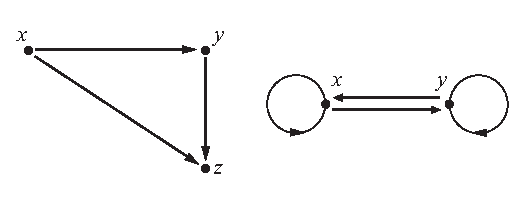
\includegraphics{figps-transitive.eps}
\end{center}
\end{figure}
\end{itemize}
%There are other properties of relations that can be studied, but we will restrict ourselves to these three, as they are the ones pertinent to the study of equivalence relations.

\begin{prog}[\textbf{Properties of Relations}] \label{prog:proprelations} \hfill \\
Let  $A = \{ a, b, c, d \}$ and let $R$ be the following relation on $A$:
\[
R = \{ (a, a), (b, b), (a, c), (c, a), (b, d), (d, b) \}.
\]
Draw a directed graph for the relation $R$ and then determine if the relation $R$ is reflexive on $A$, if the relation $R$ is symmetric, and if the relation $R$ is transitive.
\end{prog}
\hbreak

\endinput

\subsection*{Definition of an Equivalence Relation}
In mathematics, as in real life, it is often convenient to think of two different things as being essentially the same.  For example, when you go to a store to buy a cold soft drink, the cans of soft drinks in the cooler are often sorted by brand and type of soft drink.  The Coca Colas are grouped together, the Pepsi Colas are grouped together, the Dr. Peppers are grouped together, and so on.  When we choose a particular can of one type of soft drink, we are assuming that all the cans are essentially the same.  Even though the specific cans of one type of soft drink are physically different, it makes no difference which can we choose.  In doing this, we are saying that the cans of one type of soft drink are equivalent, and we are using the mathematical notion of an equivalence relation.

An equivalence relation on a set is a relation with a certain combination of properties that allow us to sort the elements of the set into certain classes.  In this section, we will focus on the properties that define an equivalence relation, and in the next section, we will see how these properties allow us to sort or partition the elements of the set into certain classes.

\begin{defbox}{equivalencerelation}{Let  $A$  be a nonempty set.  A relation  $\sim$  on the set  $A$  is an \textbf{equivalence relation}
\index{equivalence relation}%
\index{relation!equivalence}%
 provided that  $\sim$  is reflexive, symmetric, and transitive.  For  $a, b \in A$, if  $\sim$  is an equivalence relation on  $A$  and  $a \sim b$, we say that  $\boldsymbol{a}$  \textbf{is equivalent to}  $\boldsymbol{b}$.}
\end{defbox}
Most of the examples we have studied so far have involved a relation on a small finite set.  For these examples, it was convenient to use a directed graph to represent the relation.  It is now time to look at some other type of examples, which may prove to be more interesting.  In these examples, keep in mind that there is a subtle difference between the reflexive property and the other two properties.  The reflexive property states that some ordered pairs actually belong to the relation  $R$, or some elements of  $A$  are related.  The reflexive property has a universal quantifier and, hence, we must prove that for all  $x \in A$,  $x \mathrel{R} x$.  Symmetry and transitivity, on the other hand, are defined by conditional sentences.  We often use a direct proof for these properties, and so we start by assuming the hypothesis and then showing that the conclusion must follow from the hypothesis.

\begin{example}[\textbf{A Relation that Is Not an Equivalence Relation}] \hfill \\
Let  $M$  be the relation on  $\mathbb{Z}$  defined as follows:

\begin{list}{}
\item For  $a, b \in \mathbb{Z}$,  $a \mathrel{M} b$  if and only if  $a$  is a multiple of  $b$.
\end{list}
\vskip6pt
\noindent
So $a \mathrel{M} b$ if and only if there exists a  $k \in \mathbb{Z}$ such that  
$a = b k$.

\begin{itemize}
\item The relation  $M$  is reflexive on  $\mathbb{Z}$ since for each  $x \in \mathbb{Z}$,  
$x = x \cdot 1$ and, hence, $x \mathrel{M} x$.

\item Notice that  $4 \mathrel{M} 2$, but  $2 \mathrel{\not \negthickspace M} 4$.  So there exist integers  $x$  and  $y$  such that  $x \mathrel{M} y$ but  
$y \mathrel{\not \negthickspace M} x$. Hence, the relation  $M$  is not symmetric.

\item Now assume that  $x \mathrel{M} y$ and  $y \mathrel{M} z$.  Then there exist integers  $p$  and  $q$  such that
\[
x = y  p\text{  and  }y = z q .
\]
Using the second equation to make a substitution in the first equation, we see that  
%\linebreak
$x = z \left( {p q} \right)$.  Since  $p q \in \mathbb{Z}$, we have shown that  $x$  is a multiple of  $z$ and hence  $x \mathrel{M} z$.  Therefore,  $M$  is a transitive relation.
\end{itemize}
\end{example}
\noindent
The relation $M$ is reflexive on $\Z$ and is transitive, but since $M$ is not symmetric, it is not an equivalence relation on $\Z$.
\hbreak

\begin{prog}[\textbf{A Relation that Is an Equivalence Relation}] \label{prog:example-equiv} \hfill \\
Define the relation  $\sim$  on  $\Q$  as follows:  For all $a, b \in \Q$,
$a \sim b$  if and only if  $a - b \in \Z $.  For example:
\begin{itemize}
  \item  $\dfrac{3}{4} \sim \dfrac{7}{4}$ since $\dfrac{3}{4} - \dfrac{7}{4} = -1$ and $-1 \in \Z$.
  \item $\dfrac{3}{4} \not  \sim \dfrac{1}{2}$ since $\dfrac{3}{4} - \dfrac{1}{2} = \dfrac{1}{4}$ and 
$\dfrac{1}{4} \notin \Z$.
\end{itemize}
To prove that $\sim$ is reflexive on $\Q$, we note that for all $a \in \Q$, $a - a = 0$.  Since $0 \in \Z$, we conclude that $a \sim a$.  Now prove that the relation $\sim$ is symmetric and transitive, and hence, that 
$\sim$ is an equivalence relation on $\Q$.
\end{prog}
\hbreak

\endinput

\subsection*{Congruence Modulo $\boldsymbol{n}$}
One of the important equivalence relations we will study in detail is that of congruence
\index{congruence}%
 modulo  $n$.  We reviewed this relation in \typeu Activity~\ref*{PA:reviewofcongruence}.

%Let  $n \in \mathbb{N}$.  For  $a, b \in \mathbb{Z}$, we have defined  $a$  to be congruent to  $b$  modulo  $n$, denoted by  $a \equiv b \pmod n$, as follows:
%\begin{center}
%$a \equiv b \pmod n$  provided that  $n \mid \left( {a - b} \right)$.
%\end{center}
%This is equivalent to saying that  $a \equiv b \pmod n$  provided that there exists an integer  $k$  such that  $a - b = nk$.

Theorem~\ref{T:modprops} on page~\pageref{T:modprops} tells us that congruence modulo $n$ is an equivalence relation on  $\mathbb{Z}$.  Recall that by the Division Algorithm, if  $a \in \mathbb{Z}$, then there exist unique integers  $q$  and  $r$  such that
\[
a = nq + r \text{  and  }0 \leq r < n.
\]
Theorem~\ref{T:congtorem} and Corollary~\ref{C:congtorem} then tell us that  
$a \equiv r \pmod n$.  That is,  $a$  is congruent modulo  $n$ to its remainder $r$ when it is divided by  $n$.  When we use the term ``remainder'' in this context, we always mean the remainder $r$ with $0 \leq r < n$ that is guaranteed by the Division Algorithm.  We can use this idea to prove the following theorem.
%\hbreak
%
\begin{theorem} \label{T:congruence-remainder}
Let  $n \in \mathbb{N}$ and let  $a, b \in \mathbb{Z}$.  Then 
$a \equiv b \pmod n$  if and only if  $a$  and  $b$  have the same remainder when divided by  $n$.
\end{theorem}
%
\begin{myproof}
Let  $n \in \mathbb{N}$ and let  $a, b \in \mathbb{Z}$.  We will first prove that if  $a$  and  $b$  have the same remainder when divided by  $n$, then $a \equiv b \pmod n$.  So assume that  $a$  and  $b$  have the same remainder when divided by  $n$, and let  $r$  be this common remainder.  Then, by Theorem~\ref{T:congtorem},
\[
a \equiv r \pmod n \text{  and  }b \equiv r \pmod n\!.
\]
Since congruence modulo  $n$  is an equivalence relation, it is a symmetric relation.  Hence, since  $b \equiv r \pmod n$, we can conclude that  
$r \equiv b \pmod n$.  Combining this with the fact that  
$a \equiv r \pmod n$, we now have 
\[
a \equiv r \pmod n\text{  and  }r \equiv b \pmod n\!.
\]
We can now use the transitive property to conclude that  
$a \equiv b \pmod n$.  This proves that if $a$  and  $b$  have the same remainder when divided by  $n$, then  \linebreak
$a \equiv b \pmod n$.
\vskip6pt

We will now prove that if  $a \equiv b \pmod n$, then  $a$  and  $b$  have the same remainder when divided by  $n$.  Assume that  $a \equiv b \pmod n$, and let  $r$  be the least nonnegative remainder when  $b$   is divided by  $n$.  Then $0 \leq r < n$ and, by Theorem~\ref{T:congtorem},
\[
b \equiv r \pmod n\!.
\]
Now, using the facts that  $a \equiv b \pmod n$ and   
$b \equiv r \pmod n$, we can use the transitive property to conclude that
\[
a \equiv r \pmod n\!.
\]
This means that there exists an integer  $q$   such that  $a - r = nq$ or that
\[
a = nq + r.
\]
Since we already know that  $0 \leq r < n$, the last equation tells us that  $r$  is the least nonnegative remainder when  $a$  is divided by  $n$.  Hence we have proven that if  
$a \equiv b \pmod n$, then  $a$  and  $b$  have the same remainder when divided by  $n$.
\end{myproof}
\hbreak

\endinput

\subsection*{Examples of Other Equivalence Relations}
\begin{enumerate}
\item The relation $\sim$ on $\Q$ from Progress Check~\ref{prog:example-equiv} is an equivalence relation.


\item Let  $A$  be a nonempty set.  The \textbf{equality relation on}
\index{equality relation}%
\index{relation!equality}%
\index{identity relation}%
\index{relation!identity}%
  $\boldsymbol{A}$  is an equivalence relation.  This relation is also called the \textbf{identity relation on}  $\boldsymbol{A}$    and is denoted by  $I_A $, where
\[
I_A  = \left\{ {\left( {x, x} \right)   \mid x \in A} \right\}\!.
\]

\item Define the relation  $\sim$  on  $\mathbb{R}$  as follows:

\begin{list}{}
\item For  $a, b \in \mathbb{R}$,  $a \sim b$ if and only if there exists an integer  $k$  such that  $a - b = 2k\pi$.
\end{list}
\vskip10pt

We will prove that the relation  $\sim$  is an equivalence relation on  $\mathbb{R}$.  The relation  $\sim$  is reflexive on  $\mathbb{R}$ since for each  $a \in \mathbb{R}$,  
$a - a = 0 = 2 \cdot 0 \cdot \pi $.

%\vskip10pt
Now, let  $a, b \in \mathbb{R}$ and assume that  $a \sim b$.  We will prove that  $b \sim a$.  Since  $a \sim b$, there exists an integer  $k$  such that
\[
a - b = 2k\pi.
\]
By multiplying both sides of this equation by $-1$, we obtain
\[
\begin{aligned}
  ( { - 1} )( {a - b} ) &= ( { - 1} )( {2k\pi } ) \\ 
                  b - a &= 2( { - k} )\pi . \\ 
\end{aligned}
\]
Since  $ - k \in \mathbb{Z}$, the last equation proves that  $b \sim a$.  Hence, we have proven that if  $a \sim b$, then  $b \sim a$ and, therefore, the relation  $\sim$  is symmetric.

%\vskip10pt
To prove transitivity, let  $a, b, c \in \mathbb{R}$ and assume that  $a \sim b$ and  
$b \sim c$.  We will prove that  $a \sim c$.  Now, there exist integers  $k$  and  $n$  such that
\[
a - b = 2k\pi \text{  and  }b - c = 2n\pi .
\]
By adding the corresponding sides of these two equations, we see that
\[
\begin{aligned}
( {a - b} ) + ( {b - c} ) &= 2k\pi  + 2n\pi  \\ 
                    a - c &= 2( {k + n} )\pi . \\ 
\end{aligned} 
\]
By the closure properties of the integers,  $k + n \in \mathbb{Z}$.  So this proves that  
$a \sim c$ and, hence the relation  $\sim$  is transitive.

%\vskip10pt
We have now proven that  $\sim$  is an equivalence relation on  $\mathbb{R}$.  This equivalence relation is important in trigonometry.  If   $a \sim b$, then there exists an integer  $k$  such that  $a - b = 2k\pi $ and, hence,  $a = b + k( {2\pi } )$.  Since the sine and cosine functions are periodic with a period of  $2\pi $, we see that
\[
\begin{aligned}
  \sin a &= \sin( {b + k( {2\pi } )} ) = \sin b,\text{ and} \\ 
  \cos a &= \cos( {b + k( {2\pi } )} ) = \cos b. \\ 
\end{aligned} 
\]
Therefore, when  $a \sim b$, each of the trigonometric functions have the same value at  $a$  and  $b$.

\item For an example from Euclidean geometry, we define a relation  $P$  on the set  $\mathcal{L}$ of all lines in the plane as follows:

\begin{list}{}
\item For  $l_1 , l_2  \in \mathcal{L}$,  $l_1 \mathrel{P}l_2 $  if and only if  $l_1 $  is parallel to  
$l_2 $  or  $l_1  = l_2 $.
\end{list}
%\vskip6pt

We added the second condition to the definition of  $P$  to ensure that  $P$  is reflexive on  $\mathcal{L}$.  Theorems from Euclidean geometry tell us that if  $l_1 $  is parallel to  $l_2 $, then  $l_2 $  is parallel to  $l_1 $, and if $l_1 $  is parallel to  $l_2 $ and  $l_2 $  is parallel to  $l_3 $, then  $l_1 $  is parallel to  $l_3 $.  (Drawing pictures will help visualize these properties.)  This tells us that the relation  $P$  is reflexive, symmetric, and transitive and, hence, an equivalence relation on  $\mathcal{L}$.
\end{enumerate}
\hbreak

\begin{prog}[\textbf{Another Equivalence Relation}] \label{prog:anotherequiv} \hfill \\
Let  $U$  be a finite, nonempty set and let  $\mathcal{P}\left( U \right)$ be the power set of  $U$.  Recall that $\mathcal{P}\left( U \right)$ consists of all subsets of $U$. (See page~\pageref{D:powerset}.)   Define the relation  $ \approx $  on  $\mathcal{P}\left( U \right)$  as follows:

\begin{center}
For  $A, B \in \mathcal{P}\left( U \right)$,  $A \approx B$  if and only if  
$\card(A) = \card(B)$.
\end{center}
For the definition of the cardinality of a finite set, see page~\pageref{D:cardinality}.  This relation states that two subsets of $U$  are equivalent provided that they have the same number of elements. Prove that 
$\approx$ is an equivalence relation on the power set $\mathcal{P}\left( U \right)$.
\end{prog}
%\hbreak

\endinput

%
\endinput

%
%
%
%\hbreak

\begin{activity}[\textbf{Examples of Relations with Certain Properties}] \label{A:examplesofrelations} \hfill \\
Let  $A = \left\{ {1, 2, 3, 4} \right\}$.  We can define relations on the set  $A$  by simply listing the ordered pairs in the relation, and we can use digraphs to represent the relations.  For example, a relation on  $A$  that is reflexive on  $A$  but not symmetric and not transitive is  the relation in Part~(\ref{PA:directedgraphs1}) of Preview Activity~\ref{PA:directedgraphs}.  This relation is
\[
R = \left\{ {( {1, 1} ), ( {2, 2} ), ( {3, 3} ), ( {4, 4} ), ( {1, 3} ), ( {3, 2} )} \right\}.  
\]
\begin{itemize}
\item This relation is reflexive on  $A$  because  $\left( {x, x} \right) \in R$ for every  
$x \in A$. 

\item This relation is not symmetric since  $\left( {1, 3} \right) \in R$ but  
$\left( {3, 1} \right) \notin R$.  

\item This relation is not transitive since  $\left( {1, 3} \right) \in R$ and  
$\left( {3, 2} \right) \in R$, but  
\linebreak
$\left( {1, 2} \right) \notin R$.
\end{itemize}

\begin{enumerate}
\item Explain why  $R = \left\{ {\left( {1, 2} \right), \left( {2, 1} \right)} \right\}$
is a relation on  $A$  that is symmetric but not reflexive on  $A$  and not transitive .

\item Find a relation on $A$  that is transitive but neither reflexive on  $A$  nor symmetric.

\item Find a relation on $A$  that is reflexive on  $A$  and symmetric but not transitive.

\item Find a relation on $A$  that is reflexive on  $A$  and transitive but not symmetric.

\item Find a relation on $A$  that is symmetric and transitive but not reflexive on  $A$.
\end{enumerate}

The relations in this activity show that the three properties (reflexivity, symmetry, and transitivity) are independent of each other in the sense that it is possible to construct a relation that satisfies any one of the properties but not the other two.  It is also possible to construct a relation that satisfies any two of the properties but not the third.
\end{activity}
\hbreak



\begin{center}
\setlength{\unitlength}{0.5cm}
\begin{picture}(2,2)
\put(1,0){\circle*{.25}}
\put(1,1){\circle{2}}
\put(1,0){\vector(1,0){0}}
\end{picture}
\end{center} 

\begin{center}
\setlength{\unitlength}{0.5cm}
\begin{picture}(8,2)
\put(1,1){\circle*{.25}}
\put(7,1){\circle*{.25}}
\put(1.2,0.8){\vector(1,0){5.6}}
\put(6.8,1.2){\vector(-1,0){5.6}}
\end{picture}
\end{center}


\begin{center}
\setlength{\unitlength}{0.5cm}
\begin{picture}(8,6)
\put(1,5){\circle*{.25}}
\put(7,5){\circle*{.25}}
\put(7,1){\circle*{.25}}
\put(1.2,5){\vector(1,0){5.6}}
\put(7,4.8){\vector(0,-1){3.6}}
\put(1.2,5){\vector(3,-2){5.6}}
\put(0.6,5.3){$x$}
\put(7.3,5.3){$y$}
\put(7.3,0.8){$z$}
\end{picture}
\end{center} 


\begin{center}
\setlength{\unitlength}{0.5cm}
\begin{picture}(10,2)
\put(2,1){\circle*{.25}}
\put(8,1){\circle*{.25}}
\put(2.2,0.8){\vector(1,0){5.6}}
\put(7.8,1.2){\vector(-1,0){5.6}}
\put(2.2,1.6){$x$}
\put(7.6,1.6){$y$}
\put(1,1){\circle{2}}
\put(1,0){\vector(1,0){0}}
\put(9,1){\circle{2}}
\put(9,0){\vector(-1,0){0}}
\end{picture}
\end{center}
